\documentclass{article}
\usepackage[utf8]{inputenc}
\usepackage[spanish, mexico]{babel}
\usepackage[margin=0.5in]{geometry}
\usepackage{amsmath}
\usepackage{amssymb}
\usepackage{amsfonts}
\usepackage{graphicx}

\graphicspath{ {img/} }

\title{Taller de optimización}
\author{Miguel A. Gomez B.}

\begin{document}
	
	\maketitle
	\paragraph{1. Convexividad.} Graficar cada conjunto e indicar si es cerrado y/o convexo.
	\paragraph{a} $\{ x \in \mathbb{R}: x^2 - 1 = 0 \}$
	\begin{center}
		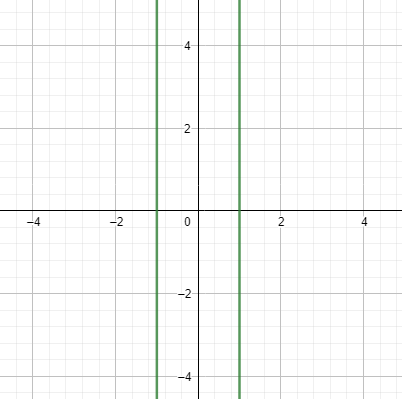
\includegraphics[width=0.3\textwidth]{a}
	\end{center}
	\paragraph{}El conjunto no es convexo y es cerrado.
	\paragraph{b} $\{ x \in \mathbb{R}: x^2 - 1 \geq 0 \}$
	\begin{center}
		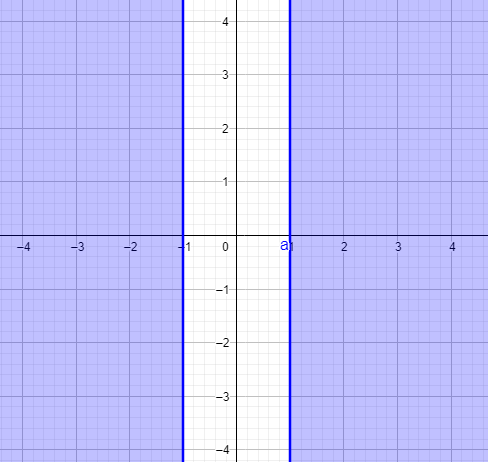
\includegraphics[width=0.3\textwidth]{b}
	\end{center}
	\paragraph{}El conjunto no es convexo y es cerrado.
	\newpage
	\paragraph{c} $\{ (x_1,x_2) \in \mathbb{R}^2: x_1 \geq x_2 \}$
	\begin{center}
		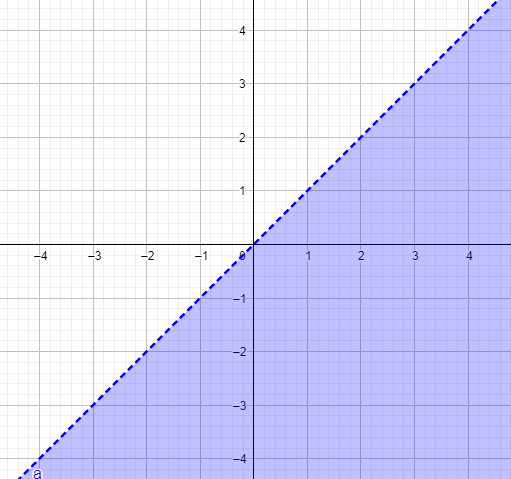
\includegraphics[width=0.3\textwidth]{c}
	\end{center}
	\paragraph{}El conjunto es convexo y no es cerrado.
	\paragraph{d} $\{ (x_1, x_2) \in \mathbb{R}^2: |x_1 - 2| < 1 \}$
	\begin{center}
		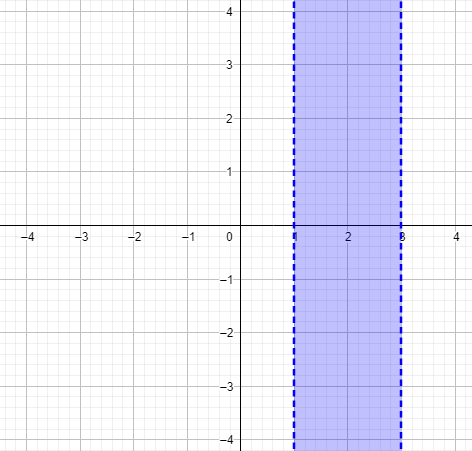
\includegraphics[width=0.3\textwidth]{d}
	\end{center}
	\paragraph{}El conjunto es convexo y no es cerrado.
	\paragraph{e} $\{ (x_1,x_2) \in \mathbb{R}^2: x_1 x_2 > 0 \}$
	\begin{center}
		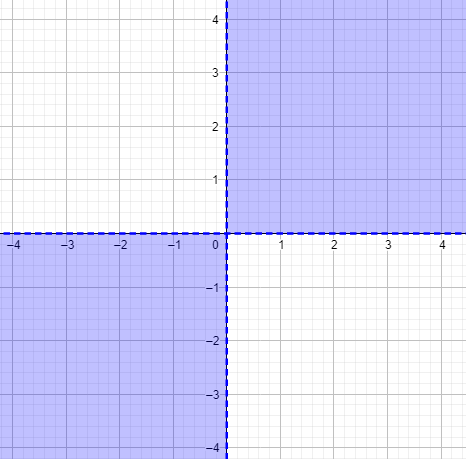
\includegraphics[width=0.3\textwidth]{e}
	\end{center}
	\paragraph{}El conjunto no es convexo y no es cerrado.
	\newpage
	\paragraph{f} $\{ (x_1,x_2) \in \mathbb{R}^2: x_1 x_2 \leq 0 \}$
	\begin{center}
		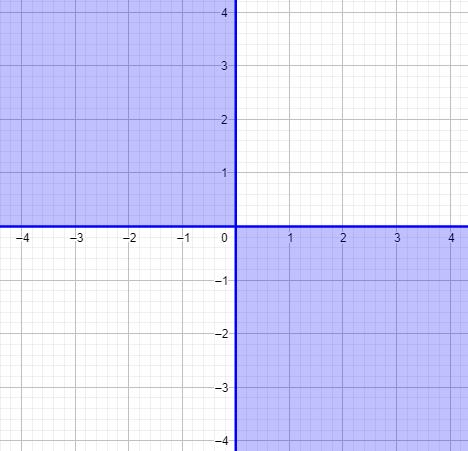
\includegraphics[width=0.3\textwidth]{f}
	\end{center}
	\paragraph{}El conjunto no es convexo y no es cerrado.
	\paragraph{g} $\{ (x_1, x_2) \in \mathbb{R}^2: x_1 x_2 = 3 \}$
	\begin{center}
		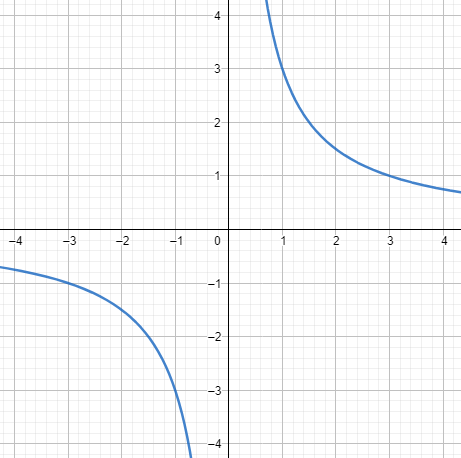
\includegraphics[width=0.3\textwidth]{g}
	\end{center}
	\paragraph{}El conjunto no es convexo y es cerrado.
	\paragraph{h} $\{ (x_1, x_2) \in \mathbb{R}^2: x^2_1 + x_2 \geq -1 \}$
	\begin{center}
		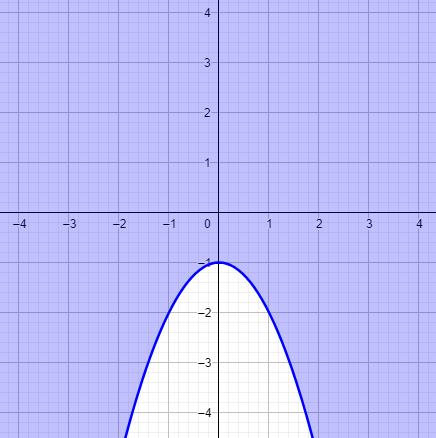
\includegraphics[width=0.3\textwidth]{h}
	\end{center}
	\paragraph{}El conjunto no es convexo y es cerrado.
	\newpage
	\paragraph{i} $\{ (x_1, x_2) \in \mathbb{R}^2: x_1 > x_2  \}$
	\begin{center}
		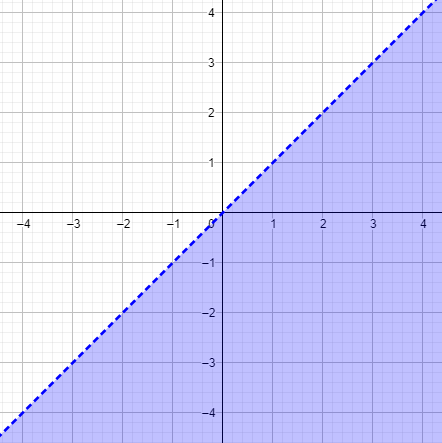
\includegraphics[width=0.3\textwidth]{i}
	\end{center}
	\paragraph{}El conjunto es convexo y no es cerrado.
	\paragraph{j} $\{ (x_1,x_2) \in \mathbb{R}^2: x_2 > x_1 \}$
	\begin{center}
		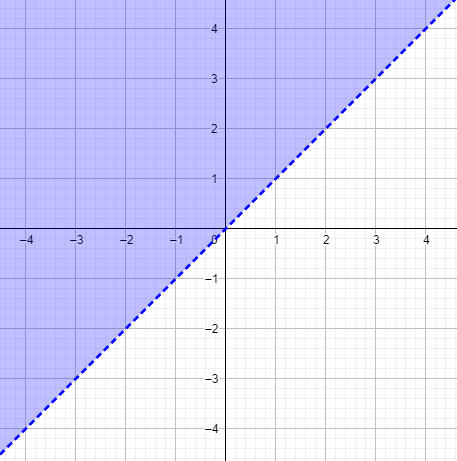
\includegraphics[width=0.3\textwidth]{j}
	\end{center}
	\paragraph{}El conjunto es convexo y no es cerrado.
	\paragraph{2. Problemas Lineales.}
	\paragraph{a} Un portafolio tiene dos tipos de inversión; en CDT's y en bonos. Un cliente desea invertir 500 dólares en el portafolio el próximo año. La inversión en CDT's tiene 5\% de interés efectivo anual y la inversión en bonos un 8\%. De acuerdo a la experiencia del asesor financiero, se recomienda invertir un máximo del 50\% de los fondos en bonos, y un mínimo de 25\% en CDT's ¿Qué valores se deben invertir en cada alternativa, para obtener el máximo beneficio?
	\paragraph{Respuesta} Definimos a $c$ y $b$ la cantidad invertida en cdt y en bonos respectivamente. Ahora definimos la función objetivo, que consiste en maximizar la ganancia, luego ésta será:
	$$Z_{max} = 0.05c + 0.08b$$
	Las recomendaciones del asesor y la restricción de cantidad de dinero del cliente se contienen en:
	\begin{itemize}
		\item La cantidad máxima que el asesor recomienda invertir en bonos no debe ser mayor al 50\% del capital, luego la restricción será:
		$$b \leq 500*0.5 = 250$$
		\item La cantidad mínima que el asesor recomienda invertir en CDT's debe ser mayor al 25\% del capital, luego la restricción será:
		$$c \geq 500*0.25 = 125 $$
		\item Existe un límite de capital que nos e puede sobrepasar de 500 dólares, luego la restricción será:
		$$c + b \leq 500$$
		\item Finalmente, la restricción del no negatividad de b.
		$$b \geq 0$$
	\end{itemize}
	\paragraph{b} Una oficina de correos requiere cantidades de empleados de tiempo completo en diferentes días de la semana. La cantidad de empleados de tiempo completo que se requiere cada día se da en la siguiente tabla. Las reglas del sindicato establece que cada empleado de tiempo completo debe trabajar cinco días consecutivos y descansa dos días. Por ejemplo un empleado que trabaja de lunes a viernes debe descansar sábado y domingo. El número de empleados que se necesita cada día está dado por: lunes: 17, Martes: 13, Miércoles: 15,Jueves: 19, Viernes: 14, Sábado: 16, Domingo: 11.
	\paragraph{Respuesta} definimos como $x_i$ La cantidad de empleados que entran a trabajar en el día $i$, luego la función objetivo consiste en minimizar:
	$$Z_{min} = x_1 + x_2 + x_3 + x_4 + x_5 + x_6 + x_7.$$
	Nótese que los empleados de un día no trabajarán pasados cinco días, para el primero por ejemplo su restricción será una suma en los siguientes días y por ende los empleados del lunes deben ser contados en las restricciones de los siguientes cinco días, para el primero:
	$$x_1 + x_7 + x_6 + x_5 + x_4 \geq 17$$
	nótese que los días $3$ y $2$ no aparecen debido a que en realidad lo que estamos contando es la cantidad de personas de los otros días que terminarían trabajando en el día lunes, es decir cinco días antes. Bajo este mismo razonamiento el sistema de inecuaciones se construye así:
	\begin{itemize}
		\item Restricción del Lunes.
		$$x_1 + x_7 + x_6 + x_5 + x_4 \geq 17$$
		\item Restricción del Martes.
		$$x_1 + x_2 + x_7 + x_6 + x_5 \geq 13$$
		\item Restricción del Miércoles.
		$$x_1 + x_2 + x_3 + x_7 + x_6 \geq 15$$
		\item Restricción del Jueves.
		$$x_1 + x_2 + x_3 + x_4 + x_7 \geq 19$$
		\item Restricción del Viernes.
		$$x_1 + x_2 + x_3 + x_4 + x_5 \geq 14$$
		\item Restricción del Sabado.
		$$x_6 + x_5 + x_4 + x_3 + x_2 \geq 16$$
		\item Restricción del Domingo.
		$$x_6 + x_7 + x_1 + x_2 + x_3 \geq 11$$
		\item Restricción de no negatividad.
		$$x_1, x_2, x_3, x_4, x_5, x_6, x_7 \geq 0$$
	\end{itemize}
	\paragraph{c} 
	La información nutricional y costos por porción de distintos alimentos se proporcionan en la siguiente tabla:
	\begin{table}[h!]
		\centering
		\begin{tabular}{c | c | c | c | c | c} 
			\hline
			\hline
			Alimento  & Costo  & Calorías & Grasa(g) & Proteína (g) & Carbohidratos (g)\\ [0.5ex] 
			\hline
			Zanahorias & 0.14 & 23 & 0.1 & 0.6 & 6 \\ 
			Papas Horneadas & 0.12 & 171 & 0.2 & 3.7 &30\\
			Pan de trigo & 0.2 & 65 & 0 & 2.2 & 13 \\
			Queso cheddar & 0.75 & 112 & 9.3 & 7 & 0 \\
			Mantequilla de maní & 0.15 & 188 & 16 & 7.7 & 2 \\
			\hline
			\hline
		\end{tabular}
	\end{table}
	\paragraph{} Se desea saber qué cantidad adquirir de cada alimento, de tal modo que se minimice el costo total de la alimentación en un día, siguendo los requisitos de la nutricionales: 
	\begin{enumerate}
		\item Las calorías consumidas deben ser al menos 2000.
		\item La grasa necesaria es de por lo menos 5$g$
		\item Se debe consumir por lo menos 100$g$ de proteína
		\item Se debe consumir al menos 250$g$ de carbohidratos.
	\end{enumerate}
	\paragraph{Respuesta} denominamos a $h$ la cantidad de zanahoria, $p$ la cantidad de porciones de papa, $t$ la cantidad de pan de trigo, $q$ la cantidad de porciones de queso cheddar y a $m$ como a la cantidad de porciones de mantequilla de maní. Como buscamos minimizar el costo, la función objetivo se define:
	$$Z_{min} = 0.14h + 0.12p + 0.2t + 0.75q + 0.15m$$
	Para definir las restricciones de aporte nutricional, debemos tener en cuenta las combinaciones lineales de las cantidades de estos alimentos, por ende para la primera restricción por ejemplo, la definimos en función de la cantidad del alimento multiplicado por el coeficiente asociado, en este caso calorías asociadas por unidad de alimento luego, la primera restricción queda definida:
	$$23h + 171p + 65t + 112q + 188m \leq 2000.$$
	Análogamente se definen el resto de restricciones, por ende las restricciones serían:
	\begin{itemize}
		\item Restricción de aporte calórico.
		$$23h + 171p + 65t + 112q + 188m \leq 2000.$$
		\item Restricción de ingesta de grasas.
		$$0.1h + 0.2p + 0t + 9.3q + 16m \leq 5.$$
		\item Restricción de ingesta de proteína.
		$$0.6h + 3.7p + 2.2t + 7q + 7.7m \leq 100.$$
		\item Restricción de aporte en carbohidratos.
		$$6h + 30p + 13t + 0q + 2m \leq 250.$$
		\item Restricción de aporte protéico.
		$$23h + 171p + 65t + 112q + 188m \leq 2000.$$
		\item Restricción de no negatividad.
		$$h,p,t,q,m \geq 0$$
	\end{itemize}
	\newpage
	\paragraph{3. Método gráfico.} Para cada problema de optimización de la forma $Ax \leq b$, $x \geq 0$, utilizar Geogebra para graficar el conjunto factible.
	\begin{itemize}
		\item Indique si el conjunto factible es acotado o no.
		\item Hallar los puntos extremos del conjunto factible.
	\end{itemize}
	\paragraph{a}.$
	A = \begin{pmatrix}
	1 & 1\\
	2 & -1\\
	0 & 1
	\end{pmatrix},
	b = \begin{pmatrix}
	4\\
	6\\
	2
	\end{pmatrix}
	$.
	\paragraph{Respuesta.} Las matrices anteriores se convierten en el conjunto de restricciones:
	$$x_1 + x_2 \leq 4,$$
	$$2x_1 - x_2 \leq 6,$$
	$$x_2 \leq 2,$$
	$$x_1, x_2 \geq 0.$$
	Obtenemos la siguiente región.
	\begin{center}
		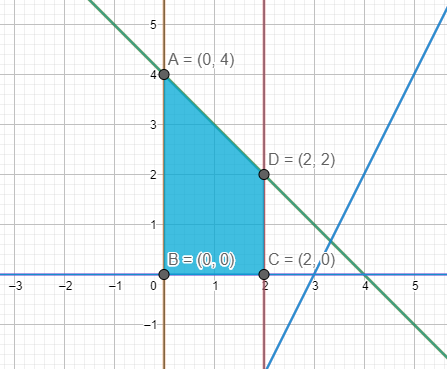
\includegraphics[width=0.6\textwidth]{3-a}
	\end{center}
	\paragraph{} El conjunto factible es acotado. y sus puntos extremos son:
	\begin{itemize}
		\item $A(0,4)$
		\item $B(0,0)$
		\item $C(2, 0)$
		\item $D(2,2)$
	\end{itemize}
	\paragraph{b}.$
	A = \begin{pmatrix}
	-1 & 0\\
	0 & -1\\
	2 & 3\\
	1 & -1
	\end{pmatrix},
	b = \begin{pmatrix}
	0\\
	0\\
	2\\
	5
	\end{pmatrix}
	$.
	\paragraph{Respuesta.} Las matrices anteriores se convierten en el conjunto de restricciones:
	$$-x_1 \leq 0 \xrightarrow{} x_1 \geq 0,$$
	$$-x_2 \leq 0 \xrightarrow{} x_2 \geq 0,$$
	$$2x_1 + 3x_2 \leq 2,$$
	$$x_1 - x_2 \leq 5,$$
	$$x_1, x_2 \geq 0.$$
	\paragraph{}Obtenemos la siguiente región factible.
	\begin{center}
		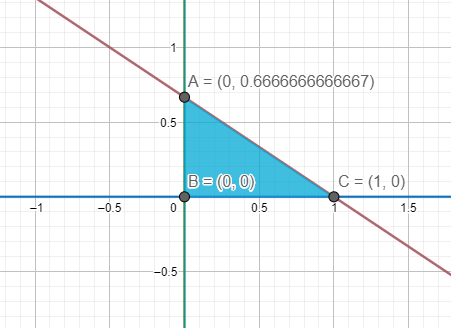
\includegraphics[width=0.6\textwidth]{3-b}
	\end{center}
	\paragraph{} El conjunto factible es acotado. Sus puntos extremos son:
	\begin{itemize}
		\item $A(0,0.6\Bar{6}).$
		\item $B(0,0).$
		\item $C(1,0).$
	\end{itemize}
	\paragraph{c}.$
	A = \begin{pmatrix}
	1 & 1\\
	-1 & -2\\
	-1 & 0
	\end{pmatrix},
	b = \begin{pmatrix}
	5\\
	-12\\
	0
	\end{pmatrix}
	$.
	\paragraph{Respuesta.} Las matrices anteriores se convierten en el conjunto de restricciones:
	$$x_1 + x_2 \leq 5$$
	$$-x_1 - x_2 \leq -12 \xrightarrow{} x_1 + x_2 \geq 12$$
	$$-x_1 \leq 0 \xrightarrow{} x_1 \geq 0$$
	$$x_1, x_2 \geq 0.$$
	\begin{center}
		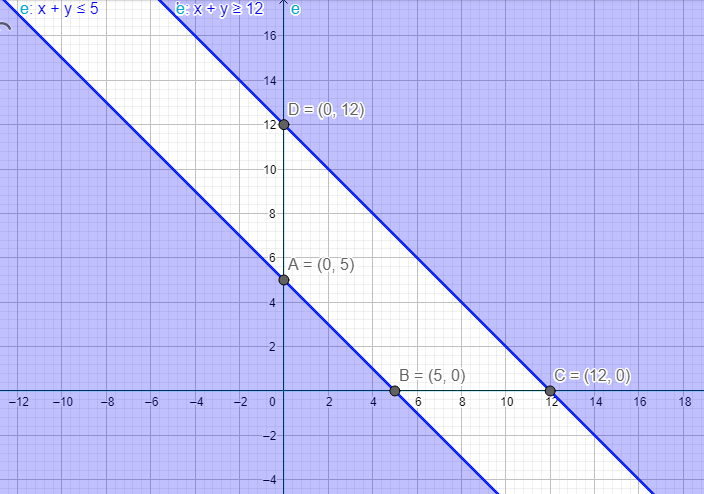
\includegraphics[width=0.5\textwidth]{3-c}
	\end{center}
	\paragraph{} Nótese que las restricciones definen dos subconjuntos en el que su intersección es vacío, luego no existe una región factible y por ende no es acotado
	\paragraph{4.} Resolver cada problema con ayuda de geogebra;
	\begin{itemize}
		\item Indique si el conjunto factible es acotado o no.
		\item Hallar los puntos extremos del conjunto factible.
		\item Determinar en que dirección aumenta o disminuye la función objetivo.
		\item Indicar si el problema tiene solución (finita) y exprese la(s) soluciones de este. 
	\end{itemize}
	\paragraph{1.}
	$$max Z = x_1 + x_2,$$
	$$x_1 \leq 4,$$
	$$x_1 + x_2 \leq 8,$$
	$$x_2 \leq 3,$$
	$$x_1, x_2 \geq 0.$$
	\paragraph{Respuesta.} Construímos el polígono.
	\begin{center}
		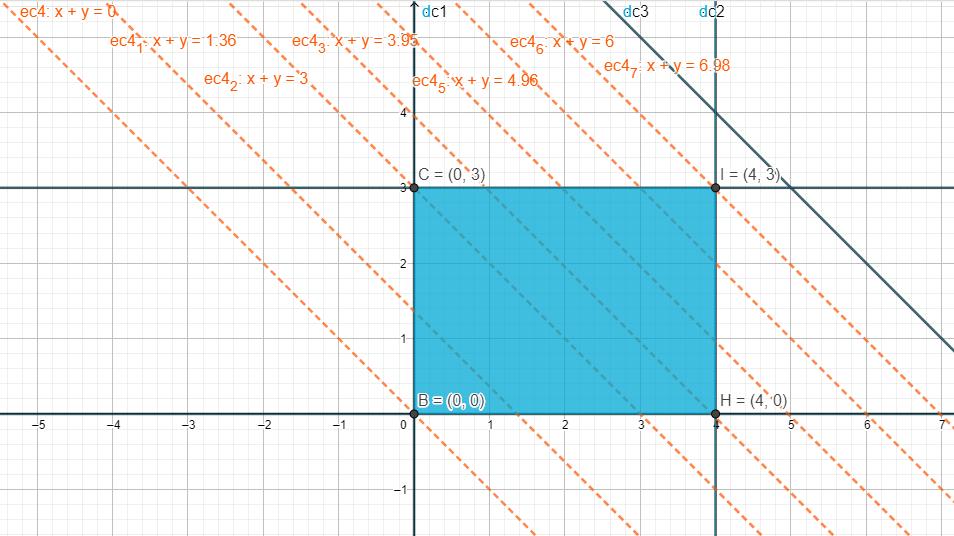
\includegraphics[width=0.5\textwidth]{4-a}
	\end{center}
	\paragraph{} El conjunto factible es acotado, sus puntos extremos se encuentran en la gráfica. A medida que se acerca al punto (4,3) la función es máxima. Y vemos que evidentemente $x + y$ va a ser mayor a medida que los valores de $x$ e $y$ sean mayores, esto es $Z(4,3) = 7$. En el resto de puntos tenemos:
	\begin{itemize}
		\item $Z(0,0) = 0$.
		\item $Z(0,3) = 3$.
		\item $Z(4,0) = 4$.
	\end{itemize}
	\paragraph{1.}
	$$min Z = -2x_1 - 4x_2,$$
	$$x_1 \leq 4,$$
	$$x_1 + x_2 \leq 8,$$
	$$x_2 \leq 3,$$
	$$x_1, x_2 \geq 0.$$
	\paragraph{Respuesta.} Construímos el polígono.
	\begin{center}
		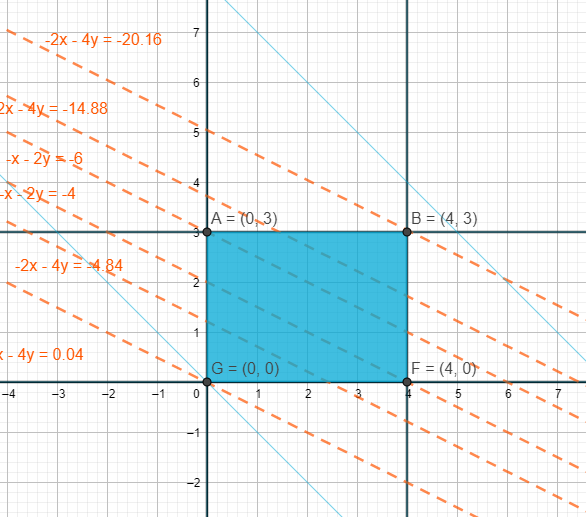
\includegraphics[width=0.5\textwidth]{4-b}
	\end{center}
	\paragraph{} El conjunto factible es acotado, sus puntos extremos se encuentran en la gráfica. A medida que se acerca al punto (4,3) la función es máxima. Y vemos que evidentemente $-2x - 4y$ va a ser menor a medida que los valores de $x$ e $y$ sean mayores, esto es $Z(4,3) = -20$. En el resto de puntos tenemos:
	\begin{itemize}
		\item $Z(0,0) = 0$.
		\item $Z(0,3) = -12$.
		\item $Z(4,0) = -8$.
	\end{itemize}
	
\end{document}
